% IEEE Paper Template for A4 Page Size (V1)
% Sample Conference Paper using IEEE LaTeX style file for A4 pagesize.
% Copyright (C) 2006-2008 Causal Productions Pty Ltd.
% Permission is granted to distribute and revise this file provided that
% this header remains intact.
%
% REVISION HISTORY
% 20080211 changed some space characters in the title-author block
%
\documentclass[10pt,conference,a4paper]{IEEEtran}
\usepackage{times,amsmath,epsfig}
\usepackage{multirow}
\usepackage{listings}
\usepackage{color}

%
% Kommandos für das Zitieren.
%
\newcommand{\zitiereSeite}[2]{\cite[][S.#2]{#1}}
\newcommand{\zitiereKapitel}[2]{\cite[][Kap.#2]{#1}}
\newcommand{\zitiere}[1]{\cite[]{#1}}

\newcommand{\vergleiche}[2]{(nach \cite[][S.#2]{#1})}

\newcommand{\sieheSeite}[2]{(siehe \cite[][S.#2]{#1})}
\newcommand{\sieheKapitel}[2]{(siehe \cite[][Kap.#2]{#1})}
\newcommand{\siehe}[1]{(siehe \cite{#1})}
%
% Kurzkommandos für Abbildungen, sowohl zum Referenzieren als auch zum Einfügen
%

%
% Kommandos für Textersetzungen, Fett, Kursiv, Mehrzeilig,...
%
\newcommand{\dbcommand}[1]{\textit{#1}}
\newcommand{\dbfile}[1]{\textit{#1}}
\newcommand{\dbname}[1]{\textbf{#1}}

\newcommand{\klasse}[1]{\textbf{#1}}
\newcommand{\member}[1]{\textit{#1}}
\newcommand{\funktion}[1]{\texttt{#1}}

\newcommand{\controller}[1]{\textbf{#1}}
\newcommand{\resource}[1]{\textit{#1}}


\definecolor{dkgreen}{rgb}{0,0.6,0}
\definecolor{gray}{rgb}{0.5,0.5,0.5}
\definecolor{mauve}{rgb}{0.58,0,0.82}

\lstset{frame=tb,
  language=Java,
  aboveskip=3mm,
  belowskip=3mm,
  basicstyle={\small\ttfamily},
  numberstyle=\tiny\color{gray},
  keywordstyle=\color{blue},
  commentstyle=\color{dkgreen},
  stringstyle=\color{mauve},
  captionpos=b
}
\renewcommand{\lstlistingname}{Ausschnitt}
\renewcommand{\lstlistlistingname}{List von \lstlistingname en}
%
\title{Dalvik VM}
%
\author{%
% author names are typeset in 11pt, which is the default size in the author block
{Reinhard Penn, Sebastian Ratzenb�ck}%
% add some space between author names and affils
}
%
\begin{document}
\maketitle
%
\begin{abstract}

\end{abstract}

%
\section{Allgemeines}
Bei Dalvik handelt es sich um eine Open Source Software die von Dan Bornstein entwickelt wurde. Benannt ist sie nach einem Fischerdorf in Eyjafj�r�ur, Island. Ver�ffentlicht wurde die Software unter Apache License 2.0. Die Ausf�hrung findet auf einem Linux Kernel statt.
\\
\\
Verwendung findet Dalvik in Googles Betriebssystem Android. Einsatz findet Dalvik hierbei als virtuelle Maschine. Der Hauptverwendungsbereich liegt im Mobilbereich, wie zum Beispiel bei Smartphones, Tablets und seit neuestem auch bei Smart Tvs und Wearables, wie Smartwatches.


\section{Architektur}
In diesem Kapitel wird die Architektur der Dalvik Virtual Machine erkl�rt. Besonderes Augenmerk wird hierbei auf den Aufbau der \member{.dex} Datei gelegt.


\subsection{Funktion}
In Android bekommt jeder Prozess seine eigene virtuelle Maschine, dabei handelt es sich um eine Dalvik VM. Sie �hnelt teilweise einer Java VM. Ein bedeutender Unterschied ist allerdings, dass eine Java VM stapelbasiert und eine Dalvik VM registerbasiert arbeitet. Diese registerbasierte Arbeitsweise lehnt sich an moderne Prozessorarchitekturen an. Sie verarbeitet Registermaschinencode, dadurch wird die Dalivk VM schneller als die Java VM und ist ressourcenschonender.
\\
\\
Ein weiterer bedeutender Unterschied liegt darin, dass eine Dalvik VM klassische Java Bibliotheken nicht unterst�tzt, zum Beispiel \member{AWT} und \member{Swing}. Es werden eigene Bibliotheken verwendet, die Apache Harmony als Grundlage verwenden.
\\
\\
Ein wichtiger Bestandteil der \member{SDK} ist das Tool \member{dx}. Es sorgt daf�r, dass Java Bin�rdaten in Dalvik Executables umgewandelt werden. Das hei�t es wandelt \member{.class} Dateien in \member{.dex} Dateien um. Bei dieser Umwandlung k�nnen auch mehrere \member{.class} Dateien zu einer \member{.dex} Datei zusammengefasst werden, beziehungsweise kann der Speicherbedarf, mithilfe von \member{.odex} Dateien optimiert werden.


\subsection{.dex Format}
In .dex Dateien werden die Klassen Definitionen und die dazugeh�rigen Daten gespeichert. Es handelt sich dabei um die ausf�hrbaren Dateien der Dalvik VM. Android Programme werden zuerst in Java Bytecode kompiliert. Dieser wird im Anschluss in Dalvik Bytecode �bersetzt. 
\\
\\
In Abbildung 1 ist der Aufbau einer .dex Datei im Vergleich zu einer .class Datei von Java zu sehen. F�r alle folgenden Listen der Datei d�rfen keine doppelten Eintr�ge vorhanden sein.

\begin{figure}
\centering
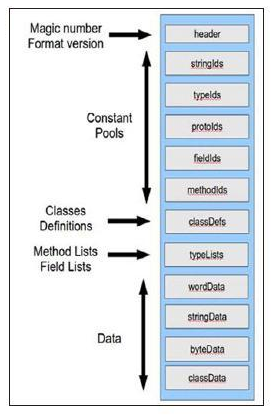
\includegraphics[width=0.4\textwidth]{DexFileFormat}
\caption{Dex Dateiformat}
\label{fig:DexFileFormat}
\end{figure}

\subsubsection{Header}
In Ausschnitt 1 ist der Header der \member{.dex} Datei zu sehen. Dabei handelt es sich um eine bestimmte Bytefolge die den Start der Datei bestimmt.

\begin{lstlisting}[float,floatplacement=H,caption=Dex Header]
ubyte[8] DEX_FILE_MAGIC = 
{ 0x64 0x65 0x78 0x0a 0x30 0x33 0x35 0x00 } 
= "dex\n035\0"

\end{lstlisting}

\subsubsection{StringIds}
Hierbei handelt es sich um eine Liste aller Strings die in der Datei verwendet werden. Die Liste muss sortiert sein und darf keine doppelten Eintr�ge enthalten. M�gliche Inhalte sind zum Beispiel konstante Strings und Funktionsnamen.

\subsubsection{TypeIds}
Dies ist eine Liste aller verwendeten Typen dieser Datei. Dazu geh�ren Klassen, Arrays, und Primitive Datentypen. Diese Liste ist nach den \member{StringIds} sortiert.

\subsubsection{ProtoIds}
In dieser Liste befinden sich alle Methoden Prototypen, die in \member{.dex} Datei verwendet werden. Die Prototypen sind prim�r anhand ihrer R�ckgabetypen sortiert und danach anhand ihrer Argumente.

\subsubsection{FieldIds}
Diese Liste enth�lt alle Felder die von der \member{.dex} Datei referenziert werden. Diese Liste wird anhand des Feldtypen und Feldnamen sortiert.

\subsubsection{MethodIds}
In der Methoden Liste werden alle von der \member{.dex} Datei referenzierten Methoden aufgelistet. Diese Liste wird nach dem Methodennamen und dem Methodenprototypen sortiert.

\subsubsection{ClassDefs}
In dieser Liste werden die Klassendefinitionen der \member{.dex} Datei angegeben. Die Liste muss so geordnet werden, dass �bergeordnete Klassen und Interfaces vor den davon ableitenden Klassen angef�hrt werden.

\subsubsection{Data}
In dem Data werden zus�tzliche Daten f�r die oben angef�hrten Listen gespeichert. Die verschiedenen Elemente haben verschiedene Alignements und padding bytes werden, wenn notwendig, eingef�gt. Des weiteren befinden sich in diesem Bereich die Daten von statisch verlinkten Dateien. Bei nicht verlinkten Dateien ist dieser Teilbereich leer.

\end{document}
